\section*{\begin{center}{Appendix E}\end{center}}
\addcontentsline{toc}{section}{Appendix E}
%$\\[0.5cm]$

\section*{Further experiment results}

\begin{figure}
    \centering
    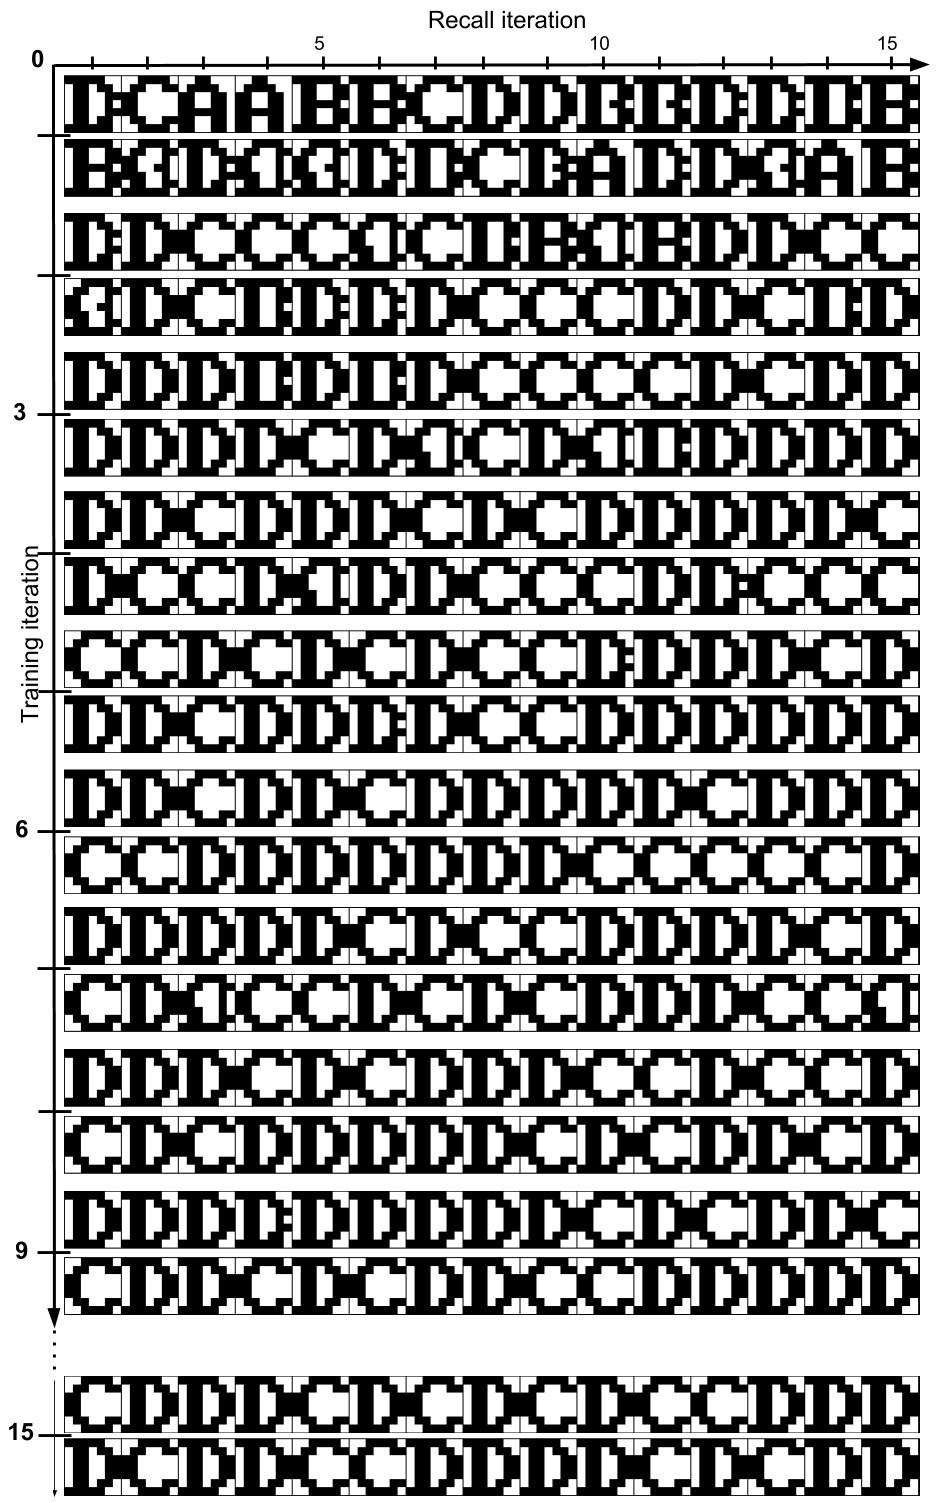
\includegraphics[width=11cm]{fig/CD-pattern-associations-async-tm0-dgw1-tau050}
    \caption{recall. async tm0 dgw1 tau050}
\end{figure}

\begin{figure}
    \centering
    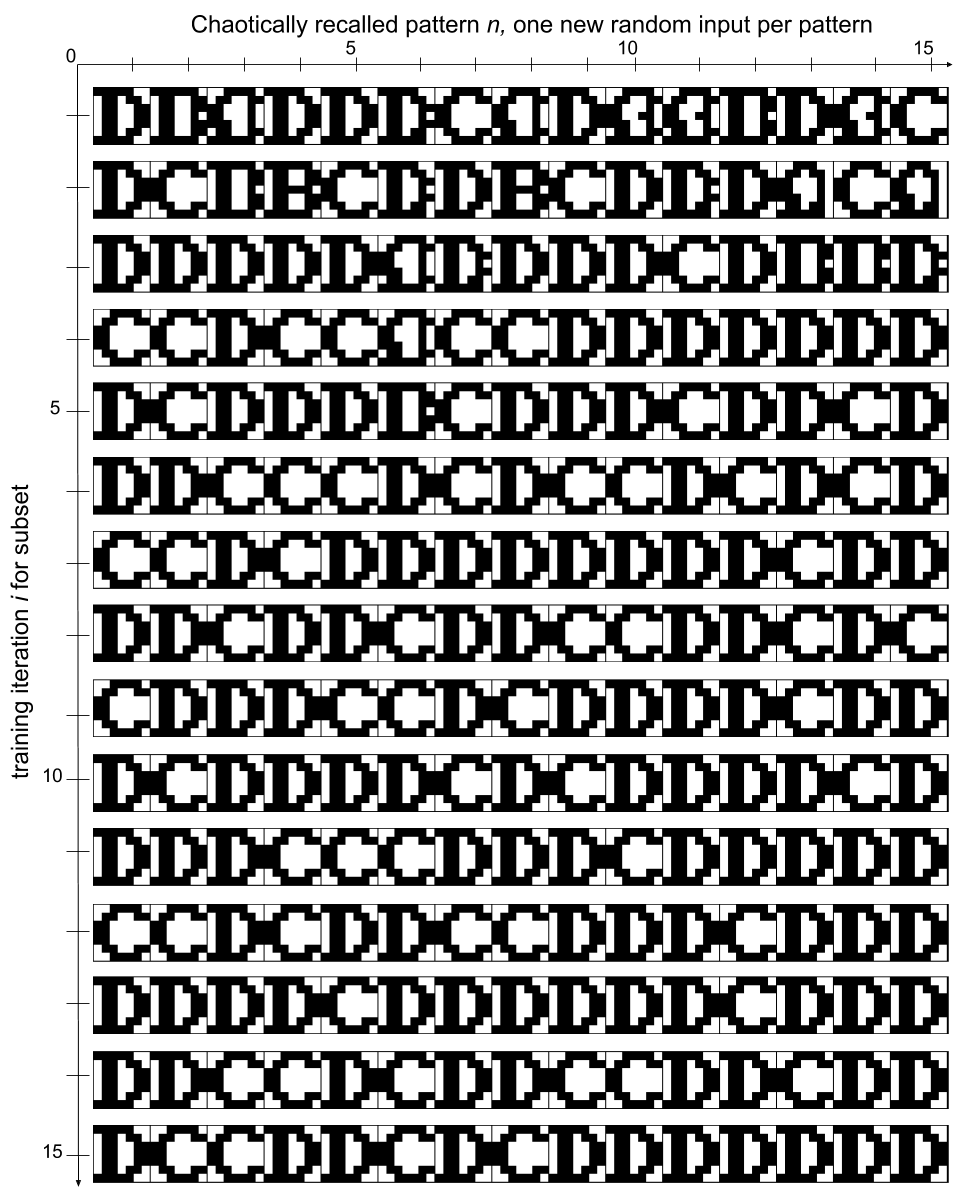
\includegraphics[width=12cm]{fig/CD-chaotic-recall-async-tm0-dgw1-tau050}
    \caption{chaotic recall. async tm0 dgw1 tau050}
\end{figure}

\subsection*{Further figures from experiment 4.2, DG-weighting}

\subsubsection{Sync.}

\begin{figure}
    \centering
    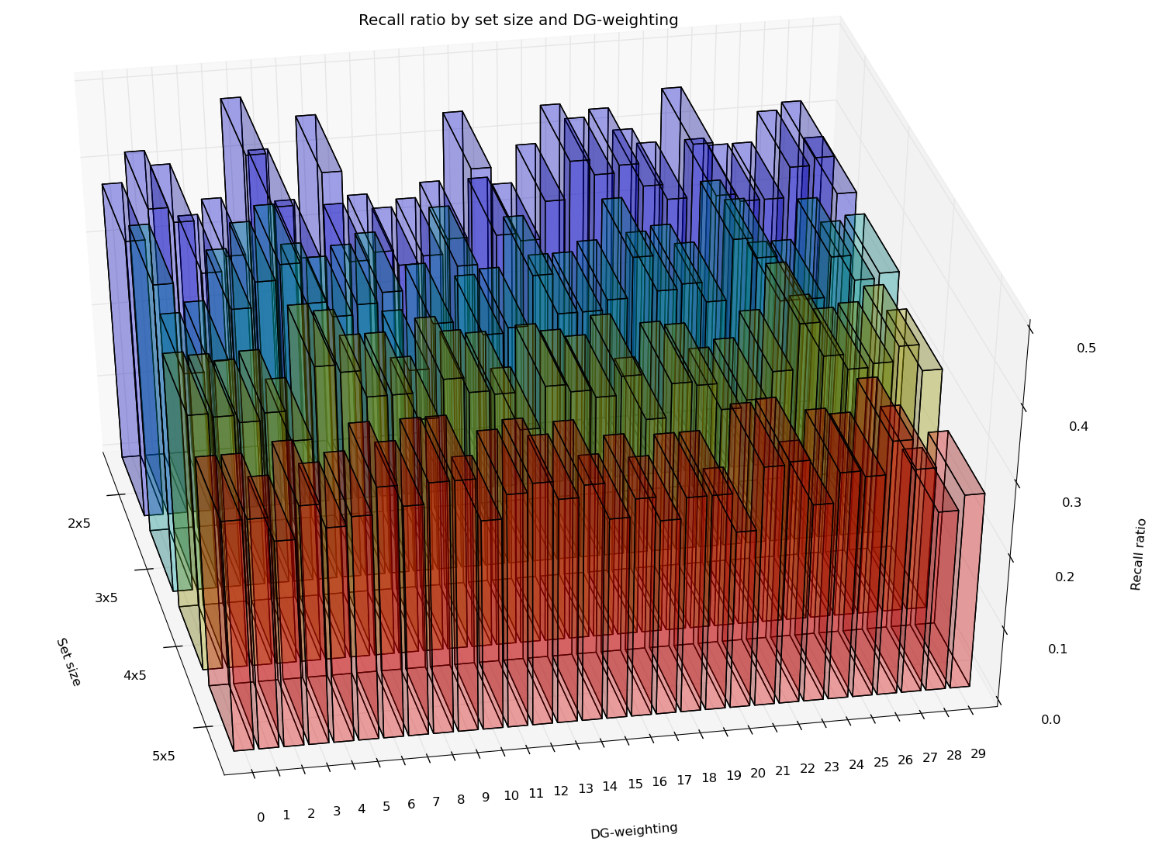
\includegraphics[width=13cm]{fig/DGWs/cut/avg_recall_ratio_by_dgw_sync_tm1_04_cut}
    \caption{PRR sync, $\tau=0.04$, turnover for every training iteration.}
    \label{fig:avg_recall_ratio_by_dgw_sync_tm1_04}
\end{figure}

\begin{figure}
    \centering
    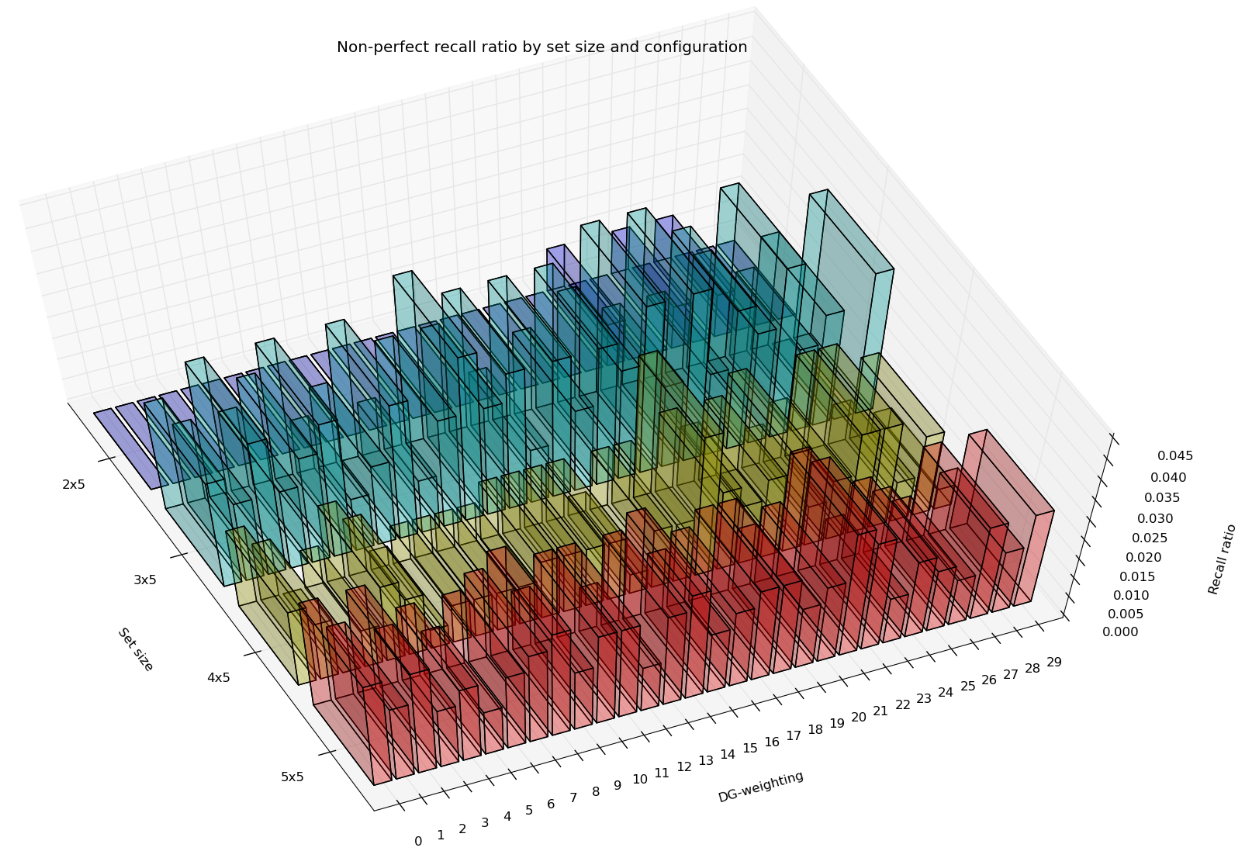
\includegraphics[width=13cm]{fig/DGWs/cut/non_perfect_recall_by_dgw_sync_tm1_04_cut}
    \caption{Spurious recall sync, $\tau=0.04$, turnover for every training iteration.}
    \label{fig:non_perfect_recall_by_dgw_sync_tm1_04}
\end{figure}


\subsubsection{Async.}

\begin{figure}
    \centering
    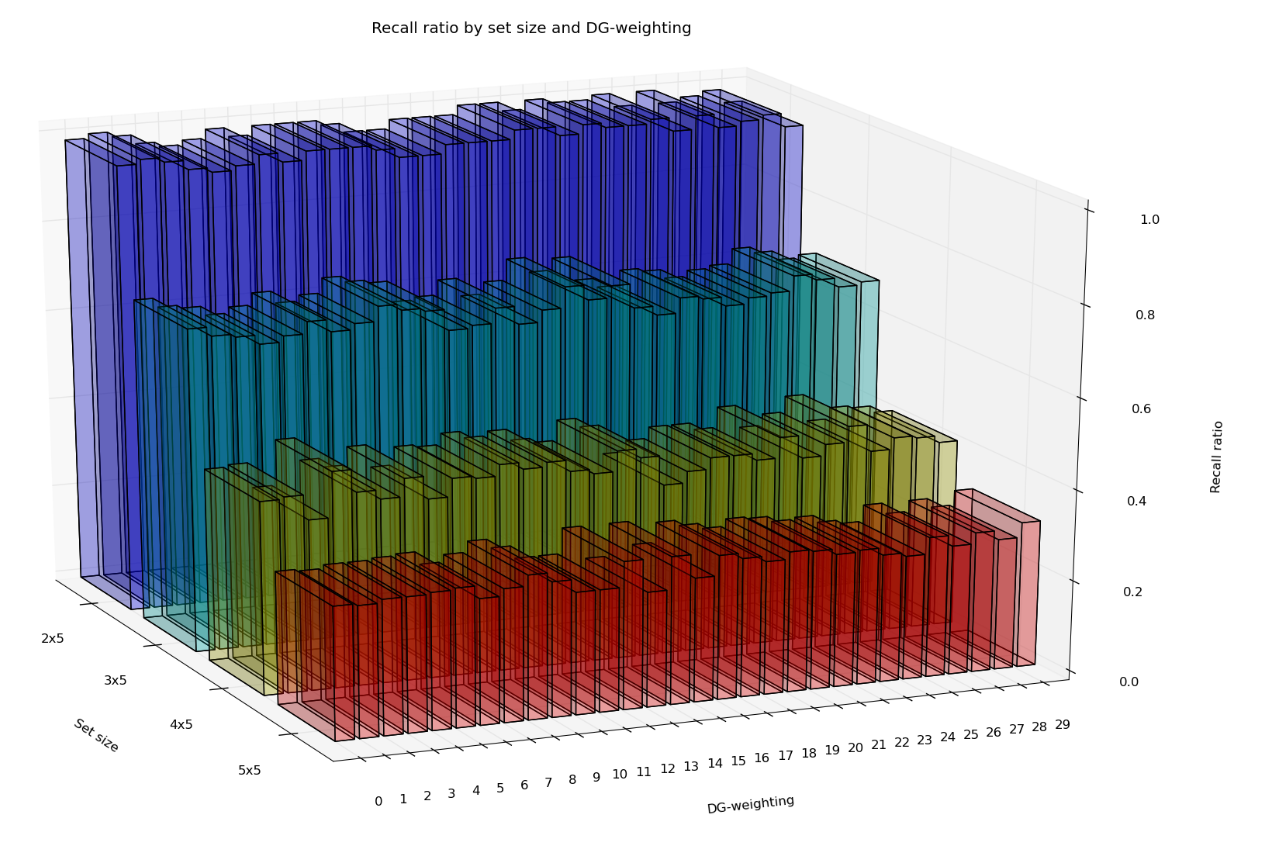
\includegraphics[width=13cm]{fig/DGWs/cut/avg_recall_ratio_by_dgw_async_tm1_04_cut}
    \caption{PRR sync, $\tau=0.04$, turnover for every training iteration.}
    \label{fig:avg_recall_ratio_by_dgw_async_tm1_04}
\end{figure}

\begin{figure}
    \centering
    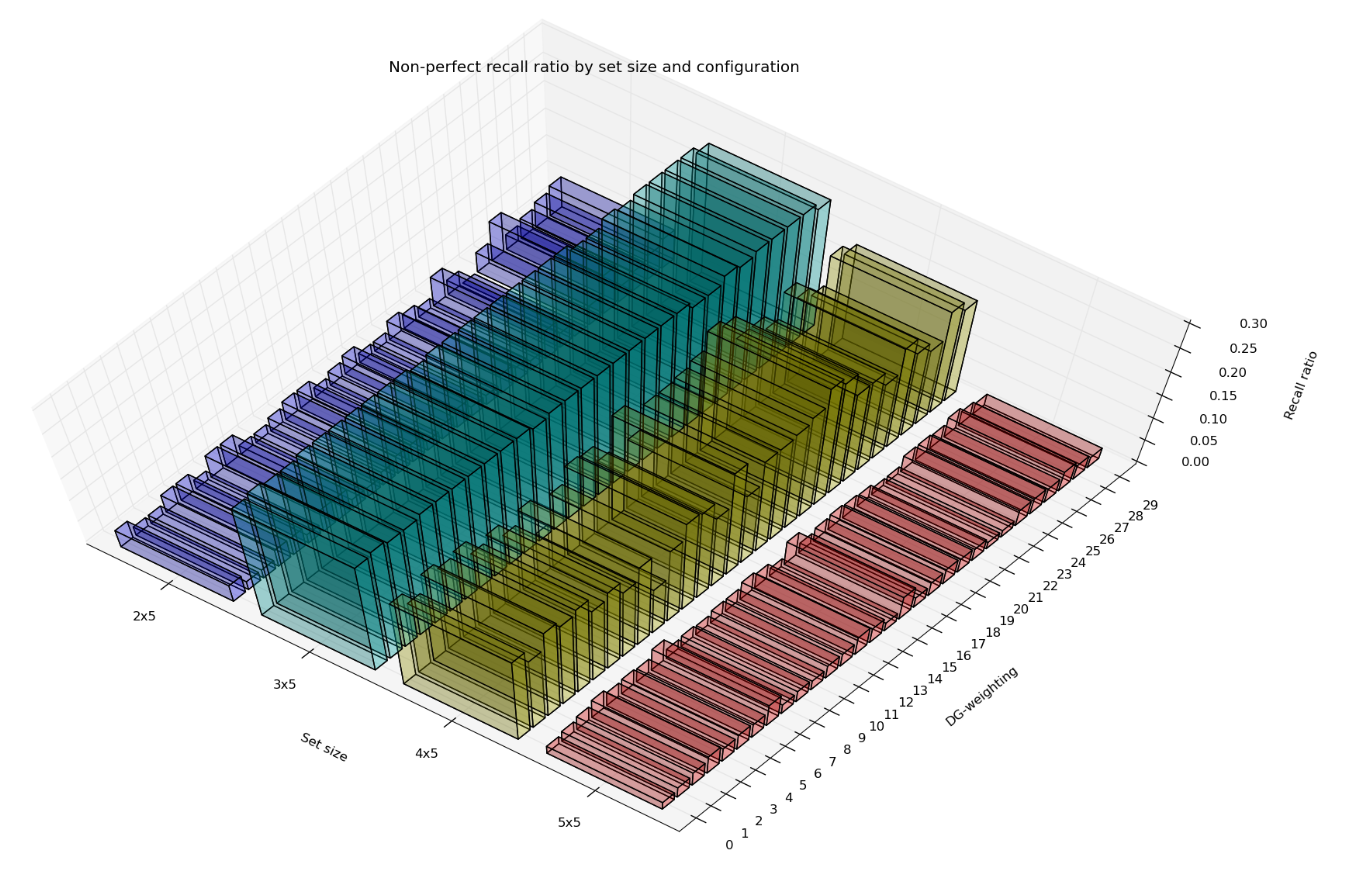
\includegraphics[width=13cm]{fig/DGWs/cut/non_perfect_recall_by_dgw_async_tm1_04_cut}
    \caption{Spurious recall sync, $\tau=0.04$, turnover for every training iteration.}
    \label{fig:non_perfect_recall_by_dgw_async_tm1_04}
\end{figure}

